\documentclass[12pt, titlepage]{article}
\usepackage{amsmath}
\usepackage{amsfonts}
\usepackage{amssymb}
\usepackage{fancyhdr}
\usepackage[bidi=basic]{babel}
\babelprovide[main,import]{hebrew}
\babelfont[hebrew]{rm}{Hadasim CLM}
\babelfont[hebrew]{sf}{Miriam Mono CLM}
\usepackage{titlesec}
\title{חשבון אינפי 2 - 01040281 \\ גליון 1}
\usepackage{graphicx}
\graphicspath{ {./images/} }
\author{יונתן אבידור - 214269565}
\titleformat{\section}{\Large\sffamily\bfseries}{\thesection}{1em}{}
\begin{document}
\maketitle
\pagestyle{fancy}
\fancyhead{}
\fancyfoot[L]{\text{214269565}}
\section*{שאלה $1$}

חשבו את האינטגרלים הבאים
\subsection*{סעיף $1$}
\[
	\int \frac{\sin x}{2+\cos x} \, dx 
    \]
\subsection*{סעיף $2$}
\[
	\int x^{2}\arcsin x^{3} \, dx 
    \]
\subsection*{סעיף $3$}
\[
	\int e^{ x }\sin5x \, dx 
    \]
\subsection*{סעיף $4$}
\[
\int e^{ 2x }\sin e^{ x } \, dx 
\]
\subsection*{סעיף $5$}
\[
	\int \frac{\log x}{x} \, dx 
    \]
\subsection*{סעיף $6$}
\[
	\int \frac{1}{x\log x} \, dx 
    \]
\subsection*{סעיף $7$}
\[
	\int \frac{x}{\sqrt{4-x^{2}}} \, dx 
    \]
\subsection*{סעיף $8$}
\[
	\int \frac{x^{2}}{x^{2}-3x-10} \, dx 
    \]
\subsection*{סעיף $9$}
\[
	\int \frac{3x-4}{x^{2}\left(x^{2}+3x+6  \right) } \, dx 
    \]
\subsection*{סעיף $10$}
\[
	\int \frac{1}{\left( x^{2}+4 \right) ^{3}} \, dx 
    \]
\section*{פתרון $1$}
\subsection*{סעיף $1$}
	\begin{gather*}
	\int \frac{\sin x}{\cos x+2} \, dx  \underset{ \begin{gathered}
	f\left( x \right) =\cos x+2 \\
	f'\left( x \right) =-\sin x
	\end{gathered} }{ = } - \int \frac{f\left( x \right)'}{f\left( x \right) } \, dx  \\
	=-\log \left| \cos x+2 \right| +C = -\log \left( \cos x+2 \right) +C
	\end{gather*}
\subsection*{סעיף $2$}
נעשה אינטגרציה בחלקים
\begin{gather*} v=\frac{x^{3}}{3} ,v'=x^{2} \\ u=\arcsin \left( x^{3} \right),  u'= 3x^{2} \frac{1}{\sqrt{1-x^{6}}} \end{gather*}
ולכן
    \begin{gather*}
	\int x^{2}\arcsin \left( x^{3} \right)   \, dx = \frac{x^{3}}{3} \arcsin \left( x^{3} \right) - \int \frac{x^{3}}{3} \cdot \frac{3x^{2}}{\sqrt{1-x^{6}}} \, dx  \\
	=\frac{x^{3}}{3}\arcsin \left( x^{3} \right) + \frac{1}{6}\int \frac{-6x^{5}}{\sqrt{1-x^{6}}} \, dx  \\
	\underset{ t=1-x^{6} }{ = } \frac{x^{3}}{3}\arcsin \left( x^{3} \right) + \frac{1}{6} \int t^{-0.5}\cdot t' \, dt = \frac{x^{3}}{3}\arcsin \left( x^{3} \right) + \frac{1}{6}\cdot 2\cdot \sqrt{t} +C\\
	= \frac{x^{3}}{3}\arcsin \left( x^{3} \right) + \frac{1}{3} \cdot \sqrt{1-x^{6}} +C \\
	=\boxed{\frac{x^{3}\arcsin \left( x^{3} \right) +\sqrt{1-x^{6}}}{3} +C}
	\end{gather*}
\subsection*{סעיף $3$}
גם כאן נעשה אינטגציה בחלקים
\begin{align*}
v=e^{ x } & v'=e^{ x } \\
u=\sin 5x & u'= 5\cos  5x 
\end{align*}
ולכן
\begin{gather*}
	\int e^{ x }\sin 5x \, dx = e^{ x } \sin 5x - \int e^{ x }5 \cos  5x\, dx 
\end{gather*}
נעשה שוב אינטגרציה בחלקים
\begin{align*}
v=e^{ x } & v'=e^{ x } \\
u=5\cos 5x & u'=-25\sin 5x
\end{align*}
וכעת
\begin{gather*}
e^{ x } \sin 5x - \int e^{ x }5 \cos  5x\, dx = e^{ x }\sin 5x - \left( e^{ x }5\cos 5x - \int -e^{ x }25\sin 5x \, dx  \right)  \\
=e^{ x }\sin 5x -\left( e^{ x }5 \cos 5x + 25\int e^{ x }\sin 5x \, dx\right) \\
= e^{ x }\sin 5x - 5e^{ x } \cos 5x - 25 \int e^{ x }\sin 5 x\, dx \\
\implies \int e^{ x }\sin 5x \, dx = e^{ x }\sin 5x - 5e^{ x } \cos 5x - 25 \int e^{ x }\sin 5 x\, dx \\
\implies 26 \int e^{ x }\sin 5x \, dx = e^{ x }\sin 5x -5 e^{ x }\cos 5x \\
\implies \boxed{\int e^{ x }\sin 5\,dx = \frac{e^{ x }\sin 5x-5e^{ x }\cos 5x}{26}}
\end{gather*}
\subsection*{סעיף $4$}
\begin{gather*}
\int e^{ 2x }\sin e^{ 2x } \, dx  = \frac{1}{2}\int 2e^{ 2x }\sin e^{ 2x } \, dx \\
\underset{ \begin{gathered}
t=e^{ 2x } \\
dt=2e^{ 2x }dx
\end{gathered} }{ = }  \frac{1}{2}\int \sin t \, dt \\
=\frac{1}{2} \left(-\cos t\right)+C \\
=\boxed{\frac{1}{2} \left( -\cos e^{ 2x } \right) +C}
\end{gather*}
\subsection*{סעיף $5$}
נשים לב ש
\[
	\frac{\log x}{x} = \log x \cdot \frac{1}{x}
    \]
שזה פונקציה כפול הנגזרת שלה, לכן מהאינטגרל המיידי $\int \left( f\left( x \right) \right)^{a}\cdot f'\left( x \right) \, dx = \frac{(f\left( x \right))^{a+1}}{a+1}$ עבור $a\neq -1$
ולכן
\[
	\int \frac{\log x}{x} \, dx  = \int \log x \cdot \frac{1}{x} \, dx  = \boxed{\frac{\left( \log x \right) ^{2}}{2}+C}
    \]
\subsection*{סעיף $6$}
קיבלנו דבר דומה רק שהפעם $a=-1$ ולכן ניזכר באינטגרל המידיי $\int \left( f\left( x \right) \right)^{-1}\cdot f'\left( x \right) \, dx=\log \left( f\left( x \right) \right)$
ולכן
\[
	\int \frac{1}{x\log x} \, dx  = \int \frac{\frac{1}{x}}{\log x} \, dx  = \boxed{\log \log x+C}
    \]
\subsection*{סעיף $7$}
\begin{gather*}
  \int \frac{x}{\sqrt{4-x^{2}}} \, dx  = \int \frac{1}{\sqrt{4-x^{2}}} x \, dx  \\
  = \int \left( 4-x^{2} \right)^{-\frac{1}{2}} x \, dx = -\frac{1}{2}\int \left( 4-x^{2} \right)^{- \frac{1}{2}}\cdot(-2x)  \, dx 
\end{gather*}
נשים לב ש
\[
	\frac{d}{dx} \left( 4-x^{2} \right) = -2x
    \]
ולכן
\[
 -\frac{1}{2}\int \left( 4-x^{2} \right)^{- \frac{1}{2}}\cdot(-2x)  \, dx  = -\frac{1}{2} \cdot \left( 2\sqrt{4-x^{2}} \right) +C = \boxed{-\sqrt{4-x^{2}}+C}
\]
\subsection*{סעיף $8$}
נבצע חילוק פולינומים 

\[
	\begin{array}{l} \\
	 	 \phantom{-}1\\
	 \phantom{-}	 \overline{x^{2}-3x-10\smash{\big{(}}}x^{2} \\
	 \phantom{-}x^{2} \\
\underline{ 	 - x^{2}-3x-10 } \\
\phantom{-~~x^{2}-}3x-10
	\end{array}
    \]
ולכן
\[
	\frac{x^{2}}{x^{2}-3x-10}=1+ \frac{3x+10}{x^{2}-3x-10}
    \]
נפרק את $x^{2}-3x-10$ ל $\left( x+2 \right)\left( x-5 \right)$ ונפרק לשברים חלקיים
\begin{gather*}
	\frac{3x+10}{x^{2}-3x-10} = \frac{A}{x+2}+ \frac{B}{x-5} \\
	\implies 3x+10 = A\left( x-5 \right) +B\left( x+2 \right)  \\
	\implies \begin{cases}
	A+B =3 \\
	-5A+2B=10
	\end{cases}
\end{gather*}
למזלנו, משוואה בשני נעלמים אנחנו יודעים לפתור גם ללא מטריצות
\begin{gather*}
	A=3-B \implies -5\left( 3-B \right) + 2B = 10  \\
	\implies -15+7B=10 \implies  7B=25 \\
	B= \frac{25}{7} \implies A = \frac{21}{7}- \frac{25}{7} = - \frac{4}{7}
\end{gather*}

ולכן
\begin{gather*}
	\int \frac{x^{2}}{x^{2}-3x-10} \, dx   \\
	= \int 1+ \frac{-4}{7}\cdot \frac{1}{x+2} + \frac{25}{7} \cdot \frac{1}{x-5} \, dx  \\
	= \int 1 \, dx- \frac{4}{7} \int \frac{1}{x+2}  \, dx   + \frac{25}{7} \int \frac{1}{x-5} \, dx  \\
	=\boxed{ x - \frac{4}{7} \cdot \log  \left| x+2 \right|   + \frac{25}{7} \cdot \log  \left| x-5 \right|  +C}
\end{gather*}
\subsection*{סעיף $9$}
נפרק לשברים חלקיים
\begin{gather*}
	\frac{3x-4}{x^{2}\left( x^{2}+3x+6 \right) } = \frac{Ax+B}{x^{2}} + \frac{Cx+D}{x^{2}+3x+6} \\
	3x-4 = \left( Ax+B \right) \cdot \left(x^{2}+3x+6  \right)  + \left( Cx+D \right)  \left( x^{2} \right)  \\
	\implies 3x-4 = Ax^{3}+3Ax^{2}+6Ax+Bx^{2}+3Bx+6B+Cx^{3}+Dx^{2} \\
	\implies 3x-4 = x^{3}\left( A+C \right)  + x^{2}\left( 3A+B+D \right)  + x\left( 6A+3B \right)  + 6B  \\
	\implies \begin{cases} 
	A+C=0 \\
	3A+B+D=0 \\
	6A+3B=3 \\
	6B=-4
	\end{cases}
\end{gather*}
גם כאן נתגבר על הדחף לדרג מטריצה ונפתור ישירות 
\begin{gather*}
	6B=-4 \implies B= -\frac{4}{6} \implies B = -\frac{2}{3}  \\
	\implies 6A-2 = 3 \implies 6A = 5 \implies A = \frac{5}{6} \\
 	 \implies \frac{5}{6} + C = 0 \implies C = -\frac{5}{6} \\
	\implies \frac{15}{6} - \frac{4}{6} + D = 0 \implies D = -\frac{11}{6}
\end{gather*}
ולכן
\begin{gather*}
\int  \frac{3x-4}{x^{2}\left( x^{2}+3x+6 \right) }\, dx 	 =\int  \frac{\frac{5x-4}{6} }{x^{2}} + \frac{\frac{-5x-11}{6} }{x^{2}+3x+6}  \, dx \\
= \frac{1}{6} \int \frac{5x-4}{x^{2}} \, dx - \frac{1}{6}\int \frac{5x+11}{x^{2}+3x+6} \, dx  \\
= \frac{5}{6} \int \frac{1}{x}  \, dx  - \frac{2}{3}\int x^{-2} \, dx - \frac{1}{6} \int \frac{5x+11}{x^{2}+3x+6} \, dx  \\
= \frac{5}{6} \log \left| x \right|   + \frac{2}{3x}  - \frac{1}{6} \int \frac{5x+11}{x^{2}+3x+6} \, dx  
\end{gather*}
נתמקד באחד שנשאר לנו $\int \frac{5x+11}{x^{2}+3x+6} \, dx$
ננסה להפוך את המונה לנגזרת של המכנה
\[
	\int \frac{5x+11}{x^{2}+3x+6} \, dx  = \frac{7}{2}\int \frac{2x+3}{x^{2}+3x+6} \, dx + \frac{5}{7}\int \frac{1}{x^{2}+3x+6} \, dx 
    \]

וכעת
\begin{gather*}
\frac{5}{2}\int \frac{2x+3}{x^{2}+3x+6} \, dx + \frac{7}{2}\int \frac{1}{x^{2}+3x+6} \, dx  \\
= \frac{5}{2}\log \left| x^{2}+3x+6 \right| + \frac{7}{2}\int \frac{1}{x^{2}+3x+6}  \, dx  
\end{gather*}
נשלים לריבוע
\begin{gather*}
 \frac{1}{x^{2}+3x+6} = \frac{1}{\left( x+ \frac{3}{2} \right)^{2}  + \frac{15}{4} }
\end{gather*}
קיבלנו ביטוי מהצורה $\frac{1}{u^{2}+a^{2}}$ כאשר $u=\left( x+\frac{3}{2} \right)$ ו $a= \frac{\sqrt{15}}{2}$, לכן
\[
\frac{7}{2}	\int  \frac{1}{\left( x+ \frac{3}{2} \right)^{2}  + \frac{15}{4} } \, dx  = \frac{7}{\sqrt{15}}\arctan \left( \frac{2x+3}{\sqrt{15}} \right) +C
\]
נחבר הכל יחדיו
\[
\boxed{ \frac{5}{6} \log \left| x \right|   + \frac{2}{3x}  - \frac{1}{6} \left( \frac{5}{2}\log \left| x^{2}+3x+6 \right| +\frac{7}{\sqrt{15}} \arctan \left( \frac{2x+3}{\sqrt{15}} \right)  \right)+C}
\]
\subsection*{סעיף $10$}
נעשה הצבה טריגונומטרית 
\[
	x=2\cdot \tan \left( \theta \right) , dx= \frac{2}{\cos ^{2}\left( \theta \right) }d\theta
    \]
נכתוב את המכנה מחדש
\[
\left( x^{2}+4^{2} \right)^{3}=,\left( 4\tan ^{2}\theta+4 \right)^{3}=\left(4\left( \tan ^{2} \theta+1 \right) \right) ^{3}=  64\sec ^{6}\theta
\]
נחזיר את זה לאינטגרל 
\[
	\int \frac{1}{64 \sec ^{6}\theta} 2\sec ^{2} \, d\theta = \int \frac{2\sec ^{2}}{64\sec ^{6}\theta} \, d\theta =  \frac{1}{32}\int \frac{1}{\sec ^{4}\theta} \, d\theta   = \frac{1}{32} \int \cos ^{4}\theta \, d\theta 
    \]
נשתמש בנוסחה מהכיתה 
\[
	\int \cos ^{n}x \, dx  = \frac{1}{n}\sin x\cos ^{n-1}x + \frac{n-1}{n}\int \cos ^{n-2}x \, dx 
    \]
עבור $n=4$
\begin{gather*}
	\frac{1}{32}\int \cos ^{4}\theta \, d\theta = \frac{1}{32}\left(  \frac{1}{4}\sin\theta \cos ^{3}\theta + \frac{3}{4}\int \cos ^{2}\theta \, d\theta   \right)
\end{gather*}
ועכשיו עבור האינטגרל שבפנים נשתמש באותה נוסחה עבור $n=2$
\[
	\int \cos ^{2}\theta \, d\theta = \frac{1}{2}\sin\theta \cos\theta + \frac{1}{2} \int \cos ^{0}\theta \, d\theta  
    \]
מכיוון ש $\cos ^{0}=1$ אנחנו מקבלים את האינטגרל המיידי $\int 1 \, d\theta=\theta$
נחבר את החלקים
\begin{gather*}
	\frac{1}{32}\left( \frac{1}{4}\sin\theta \cos ^{3}\theta+\frac{3}{4}\left( \frac{1}{2}\sin\theta \cos\theta+\frac{1}{2}t \right)  \right)   \\
	= \frac{1}{128}\sin\theta \cos ^{3}\theta+ \frac{3}{256}\sin\theta \cos\theta +\frac{3}{256}t+C
\end{gather*}
נחזיר לביטוי של $x$ 
\[
	x=2\tan \theta \implies \tan  \theta  =\frac{x}{2}
    \]
נרצה למצוא לפי זה את $\cos\theta,\sin\theta$
נצייר את המשולש עם זווית $\theta$, צלע "ממול" $x$ וצלע "ליד" $2$ (לקח לי חצי שעה לעשות את זה בtikz)\\
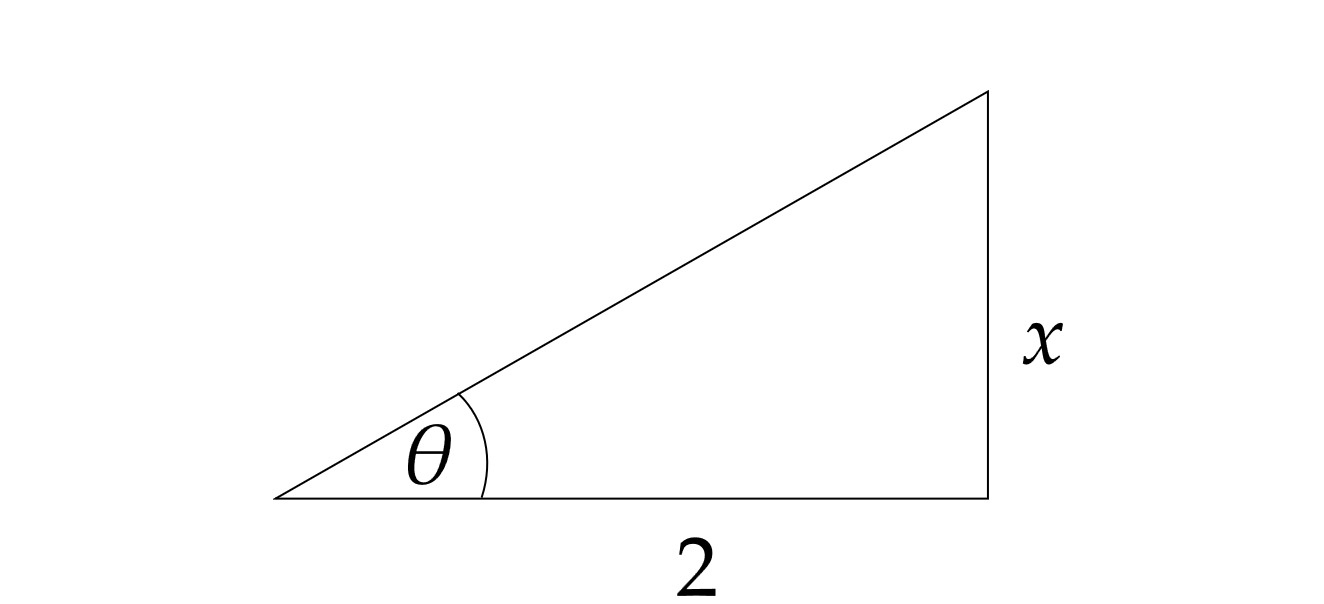
\includegraphics[width=\textwidth]{first-image.png}
לפי משפט פיתגורס, היתר הוא $\sqrt{x^{2}+4}$, לכן
\begin{gather*}
	\sin\theta = \frac{x}{\sqrt{x^{2}+4}} \\
	\cos\theta=\frac{2}{\sqrt{x^{2}+4}} \\
	\theta = \arctan \left( \frac{x}{2} \right) 
\end{gather*}
נציב במה שקיבלנו
	 \begin{gather*}
	 \frac{1}{128}\sin\theta \cos ^{3}\theta+ \frac{3}{256}\sin\theta \cos\theta +\frac{3}{256}t+C  \\
	 = \frac{1}{128}\left( \frac{x}{\sqrt{x^{2}+4}} \cdot\frac{8}{\sqrt{x^{2}+4}^{3}} \right)  + \frac{3}{256} \left( \frac{x}{\sqrt{x^{2}+4}} \cdot\frac{2}{\sqrt{x^{2}+4}} \right)  \\
	 + \frac{3}{256}\arctan \left( \frac{x}{2} \right) +C \\
	 = \frac{8x}{128\left( x^{2}+4\right)^{2} } + \frac{6x}{256\left( x^{2}+4 \right) }+ \frac{3}{256}\arctan \left( \frac{x}{2} \right) +C \\
	 = \boxed{\frac{x}{16\left( x^{2}+4 \right) ^{2}}+ \frac{3x}{128\left( x^{2}+4 \right) ^{2}}+\frac{3}{256}\arctan \left( \frac{x}{2}+C \right)  }
\end{gather*}
\section*{תרגיל 2}
ההצבה $t=\tan \frac{x}{2}$ מאפשרת לנו להפוך פונקציות רציונליות עם $\sin x$ ו-$\cos x$ לפונקציה רציונלית סטנדרטית.
\subsection*{סעיף א'}
מצאו את $\sin x$ ואת $\cos x$ כביטוי של $t$
\subsection*{סעיף ב'}
מצאו את $dx$ כביטוי של $t$ ו-$dt$
\subsection*{סעיף ג'}
השתמשו בשיטת ההצבה הזו על מנת להראות כי
\[
	\int \frac{1}{2+\cos x+\sin x} \, dx = \sqrt{2} \arctan \left( \frac{\tan \frac{x}{2}+1}{\sqrt{2}} \right) 
    \]
\section*{פתרון 2}
\subsection*{סעיף א'}
בדומה למה שעשינו באינטגרל העשירי (אבל הפוך) מהשאלה הקודמת, נצייר משולש שזוויתו $\frac{x}{2}$, הבסיס הרחוק יהיה $t$ והבסיס הקרוב יהיה $1$. (ממש השתלם ללמוד tikz) \\
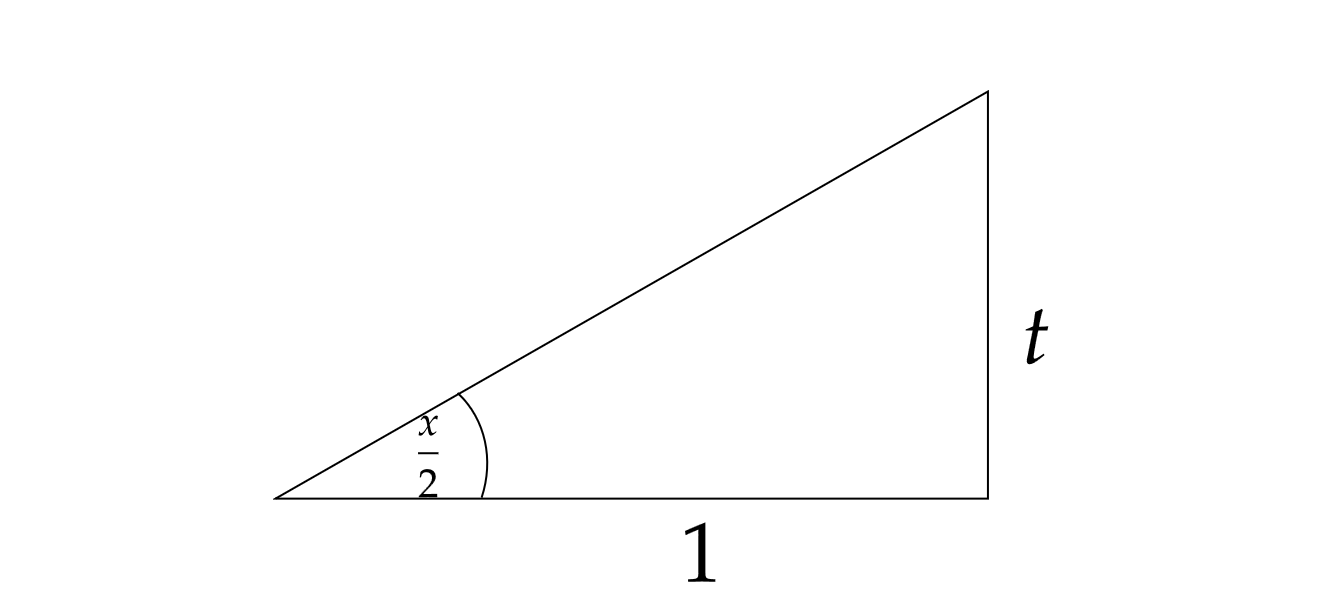
\includegraphics[width=\textwidth]{second-image.png}
לפי משפט פיתגורס, אורך היתר הוא $\sqrt{t^{2}+1}$
לכן
\begin{gather*}
	\sin \frac{x}{2}= \frac{t}{\sqrt{t^{2}+1}} \\
	\cos \frac{x}{2}= \frac{1}{\sqrt{t^{2}+1}}
\end{gather*}
נשתמש בזהויות עבור זווית כפולה ונקבל
\begin{gather*}
	\sin x = \frac{2t}{\sqrt{t^{2}+1}} \frac{1}{\sqrt{t^{2}+1}}= \frac{2t}{t^{2}+1} \\
	\cos x= \frac{1}{t^{2}+1}- \frac{t^{2}}{t^{2}+1} = \frac{1-t^{2}}{t^{2}+1}
\end{gather*}
\subsection*{סעיף ב'}
ראשית, נכתוב את $x$ כביטוי של $t$
\[
	t= \tan \left( \frac{x}{2} \right) \implies 2\arctan \left( t \right)  = x
    \]
נגזור ונקבל כי
\[
	\boxed{dx=  \frac{2}{t^{2}+1}dt}
    \]
\subsection*{סעיף ג'}
נציב באינטגרל את הנוסחאות שמצאנו בסעיפים הקדומים
\begin{gather*}
		\int \frac{1}{2+\cos x+\sin x} \, dx =  \int \frac{1}{2+\frac{1-t^{2}}{t^{2}+1}+\frac{2t}{t^{2}+1}} \frac{2}{t^{2}+1}\,dt  \\
		=2\int \frac{1}{2t^{2}+2+1-t^{2}+2t} \, dt \\
		= 2\int \frac{1}{t^{2}+2t+3} \, dt \\
		= 2\int \frac{1}{\left( t+1 \right)^{2}+2 } \, dt
\end{gather*}

קיבלנו ביטוי מהצורה $\frac{1}{u^{2}+a^{2}}$ כאשר$u=t+1$ו $a=\sqrt{2}$, לכן
\[
	2\int \frac{1}{\left( t+1 \right) ^{2}+2} \, dt = \sqrt{2}\arctan \left( \frac{t+1}{\sqrt{2}} \right) +C
    \]
נחזיר $t=\tan \frac{x}{2}$ ונקבל
\[
	\sqrt{2}\arctan \left( \frac{\tan \frac{x}{2}+1}{\sqrt{2}} \right) 
    \]
כנדרש
$\blacksquare$
\end{document}
